%20 min preso!
\documentclass[xcolor=table]{beamer}
\usepackage{beamerthemesplit}
\usepackage{wrapfig}
\usetheme{SPbGU}
\usepackage{pdfpages}
\usepackage{amsmath}
\usepackage{cmap}
\usepackage[T2A]{fontenc}
\usepackage[utf8]{inputenc}
\usepackage[english]{babel}
\usepackage{indentfirst}
\usepackage{amsmath}
\usepackage{tikz}
\usetikzlibrary{automata,positioning}
\usepackage{multirow}
\usepackage[noend]{algpseudocode}
\usepackage{algorithm}
\usepackage{algorithmicx}
\usepackage{fancyvrb}
\usepackage{subcaption}
\usepackage{listings}
%\usepackage{multicol}
\usetikzlibrary{calc}
\usetikzlibrary{shapes,arrows}
\usetikzlibrary{arrows,automata}
\usetikzlibrary{positioning}

\usepackage{tabularx}
\newcolumntype{Y}{>{\raggedleft\arraybackslash}X}


\newtheorem{mytheorem}{Theorem}
\renewcommand{\thealgorithm}{}

\newcommand{\tikzmark}[1]{\tikz[overlay,remember picture] \node (#1) {};}
\def\Put(#1,#2)#3{\leavevmode\makebox(0,0){\put(#1,#2){#3}}}

\tikzset{
    state/.style={
           rectangle,
           rounded corners,
           draw=black, very thick,
           minimum height=2em,
           inner sep=2pt,
           text centered,
           },
    horiz/.style={
                  % font=\tiny,
              inner sep=3pt,
              font=\bf

                  } ,
    point/.style={
                  circle,
                  minimum width = 5pt,
                  fill
                  },
}




\beamertemplatenavigationsymbolsempty

\title[Parsing Techniques for CFPQ]{Parsing Techniques for Contex-Free Path Querying}
%\subtitle[YaccConstructor]{Parsing techniques for graph analysis}
% То, что в квадратных скобках, отображается в левом нижнем углу.
\institute[JetBrains Research]{
JetBrains Research, Programming Languages and Tools Lab  \\
Saint Petersburg University
}

% То, что в квадратных скобках, отображается в левом нижнем углу.
\author[Semyon Grigorev]{\textbf{Semyon Grigorev}\\ \href{mailto:s.v.grigoriev@spbu.ru}{s.v.grigoriev@spbu.ru}\\
\href{mailto:Semen.Grigorev@jetbrains.com}{Semen.Grigorev@jetbrains.com}}

\date{April 05, 2019}

\begin{document}
{
\begin{frame}[fragile]
%  \begin{table}
%  \centering
%  \begin{tabularx}{\linewidth}{YcX}
%    
\includegraphics[height=1.5cm]{pictures/jetbrainsResearch.pdf} \hfill
%    & \begin{minipage}[t]{0.3\textwidth}\center \vspace{-1cm}
%      \end{minipage}
%    & \hfill 
\includegraphics[height=1.5cm]{pictures/SPbGU_Logo.png}
%  \end{tabularx}
%  \end{table}
  \titlepage
\end{frame}
}

%\begin{frame} \frametitle{Programming Languages and Tools Lab}
%    \begin{itemize}
%      \item \url{https://research.jetbrains.org/groups/plt_lab}
%    \end{itemize}
%\end{frame}




\begin{frame} \frametitle{Formal language constrained path querying}
\begin{itemize}
\item Finite directed edge-laballed graph $\mathcal{G} = (V,E,L)$
\item The path is a world over $L$: $\omega(p) = \omega(v_0 \xrightarrow{l_0} v_1 \xrightarrow{l_1} \dots \xrightarrow{l_{n-1}} v_n ) = l_0 \cdot l_1 \cdot \ldots \cdot l_{n-1}$
\item The language $\mathcal{L}$ (over $L$)
\end{itemize}
\pause
\begin{itemize}
  \item Reachability problem: $Q=\{(v_i,v_j) \ | \ \exists p = v_i \dots v_j, \omega(p) \in \mathcal{L}\}$
  \item Path querying problem: $Q=\{p \ | \ \omega(p) \in \mathcal{L}\}$
  \begin{itemize}
    \item Single path, all paths, shortest path \dots
  \end{itemize}
\end{itemize}

\end{frame}

\begin{frame} \frametitle{Context-Free path querying}
\begin{itemize}
\item $\mathcal{L}$ is a context-free language
\item $G_{\mathcal{L}} = (N,\Sigma,R,S)$
\item Reachability problem: $Q=\{(v_i,v_j) \ | \ \exists p = v_i \dots v_j, S \xrightarrow[G_L]{*} \omega(p) \}$
\item Path querying problem: $Q=\{p \ | \ \omega(p) \in \mathcal{L}\}$
\end{itemize}

\end{frame}

\begin{frame} \frametitle{Example of CFPQ}

\begin{center}
  \begin{tabular}{  c  c  }
      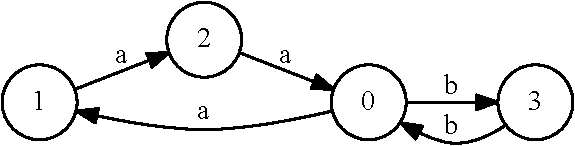
\includegraphics[width=0.45\textwidth]{pictures/input.pdf}
      &
  $

  \begin{array}{rl}
     0:& S \rightarrow a \ S \ b \\
     1:& S \rightarrow Middle \\
     2:& Middle \rightarrow a \ b
  \end{array}

  $
  \\
  Input graph
  &
  Query: language $\{a^nb^n \ | \ n > 0 \}$

  \end{tabular}
\end{center}
\vspace{0.5cm}
Paths: \\
$2 \xrightarrow{a} 0 \xrightarrow{b} 3$ \\
$1 \xrightarrow{a} 2 \xrightarrow{a} 0 \xrightarrow{b} 3 \xrightarrow{b} 0$ \\
$p_1 = 0 \xrightarrow{a} 1 \xrightarrow{a} 2 \xrightarrow{a} 0 \xrightarrow{b} 3 \xrightarrow{b} 0 \xrightarrow{b} 3$ \\
$p_2 = 0 \xrightarrow{a} 1 \xrightarrow{a} 2 \xrightarrow{a} 0 \xrightarrow{a} 1 \xrightarrow{a} 2 \xrightarrow{a} 0 \xrightarrow{b} 3 \xrightarrow{b} 0 \xrightarrow{b} 3 \xrightarrow{b} 0 \xrightarrow{b} 3 \xrightarrow{b} 0$ \\
$\dots$

\end{frame}


\begin{frame} \frametitle{Applications}
\begin{itemize}
\item Graph data bases querying \\
Yann ...
\item Static code analysis \\
Reps CFL reachability
\item \dots
\end{itemize}
\end{frame}

\begin{frame} \frametitle{Graph data bases querying}

  \begin{minipage}[m]{0.45\linewidth}
  \raisebox{-0.5\totalheight}{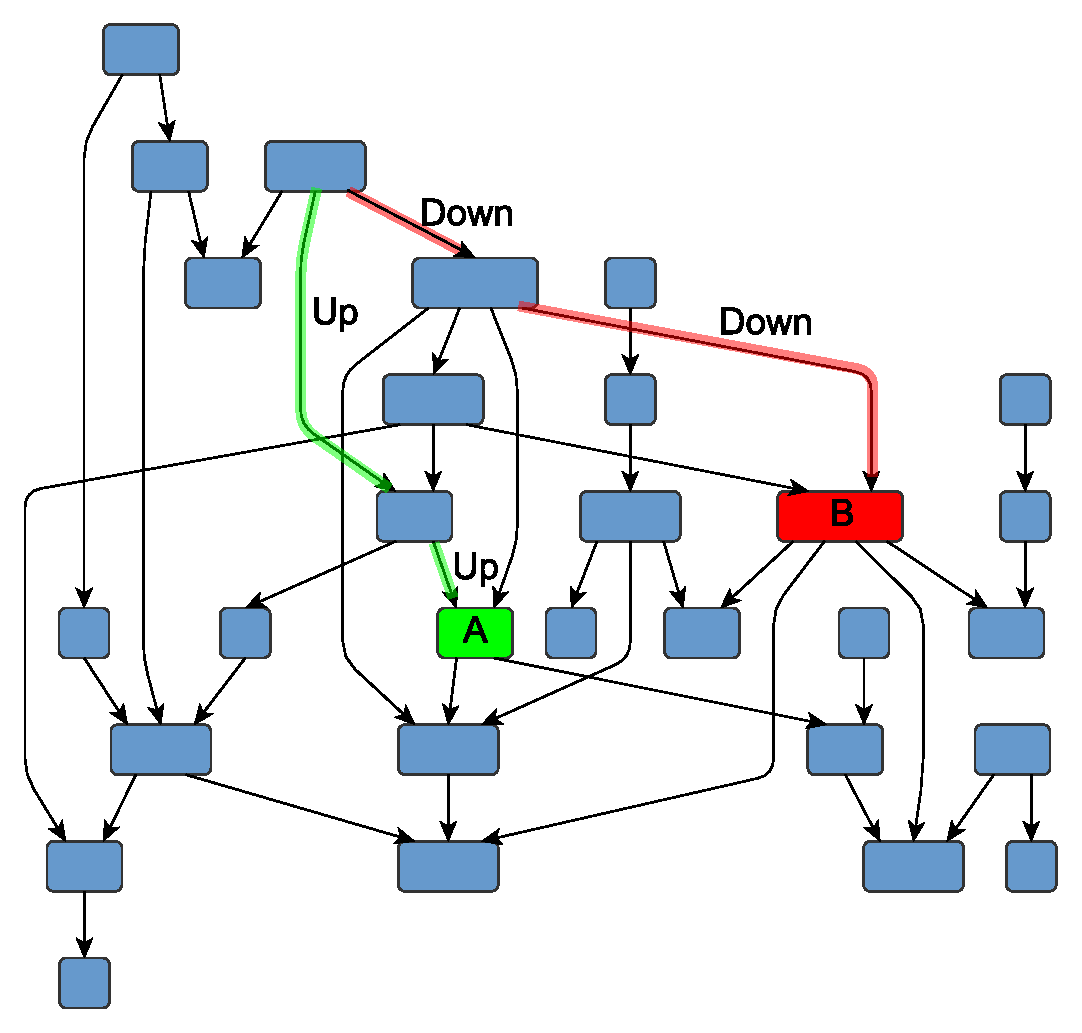
\includegraphics[width=\textwidth]{pictures/hierarchical.pdf}}
  \end{minipage}\hfill
  \begin{minipage}[m]{0.5\linewidth}
  Navigation through a graph
  \begin{itemize}
        \item Are nodes A and B on the same level of hierarchy?
        \item Is there a path of form $\textbf{Up}^n \, \textbf{Down}^n$?
        \item Find all paths of form $\textbf{Up}^n \, \textbf{Down}^n$ which start from the~node A
  \end{itemize}

  \end{minipage}


\end{frame}

\begin{frame}[fragile]
  \frametitle{Context-Free Path Querying}
    \begin{itemize}
        \item \emph{Sevon P., Eronen L.} ``Subgraph queries by context-free grammars.'' 2008
        \item \emph{Hellings J.} ``Conjunctive context-free path queries.'' 2014
        \item \emph{Zhang X. et al.} ``Context-free path queries on RDF graphs.'' 2016
    \end{itemize}
\end{frame}


\begin{frame}[fragile] \frametitle{Static code analysis}
  \begin{minipage}[t]{0.45\textwidth}
    \vspace{-7.5cm}
    \lstset{language=C,basicstyle=\small}
    \begin{lstlisting}
    int id(int u)
    {
      v = u;
      return v;
    }
    int main()
    {
      //taint
      int x;
      int z, y;
      //untaint
      int t;
      z = id(x);
      t = id(y);
    }
  \end{lstlisting}
\end{minipage}
~
\begin{minipage}[t]{0.45\textwidth}
  \begin{tikzpicture}[shorten >=1pt, >=stealth', node distance=1.9cm,on grid,auto]
  \tikzstyle{none} = [draw=none, minimum height=0.4cm, minimum width=1cm]
     \node[none]  (a)              {\emph{taint}};
     \node[state] (b) [below of=a] {$x$};
     \node[state] (d) [below of=b] {$u$};
     \node[state] (c) [below of=d] {$y$};
     \node[state] (e) [right of=d] {$v$};
     \node[state] (f) [above of=e] {$z$};
     \node[state] (g) [below of=e] {$t$};
     \node[none]  (h) [below of=g] {\emph{untaint}};
     \path[->]
      (a) edge[horiz] node[left]  {save} (b)
      (b) edge[horiz] node[left]  {$\boldsymbol{call\_id}_1$} (d)
      (c) edge[horiz] node        {$\boldsymbol{call\_id}_2$} (d)
      (d) edge[horiz] node        {save} (e)
      (e) edge[horiz] node[right] {$\boldsymbol{ret\_id}_1$} (f)
      (e) edge[horiz] node        {$\boldsymbol{ret\_id}_2$} (g)
      (g) edge[horiz] node        {save} (h)

      ;
  \end{tikzpicture}

\end{minipage}

\end{frame}

\begin{frame}
  \frametitle{Static code analysis (Language Reachability Framework)}
    \begin{itemize}
        \item \emph{Thomas Reps et al.} ``Precise interprocedural dataflow analysis via graph reachability.'' 1995
        \item \emph{Dacong Yan et al.} ``Demand-driven context-sensitive alias analysis for Java.'' 2011
        \item \emph{Jakob Rehof and Manuel Fahndrich.} ``Type-base flow analysis: from polymorphic subtyping to CFL-reachability.'' 2001
        \pause
        \item \emph{Qirun Zhang and Zhendong Su.} ``Context-sensitive data-dependence analysis via linear conjunctive language reachability.'' 2017
    \end{itemize}
  \end{frame}



\begin{frame} \frametitle{Parsing algorithms for CFPQ}
\begin{itemize}
\item Structural representation of results
\item Number of algorithms with different properties
\item Number of theoretical results
\end{itemize}
\end{frame}

\begin{frame}[fragile] \frametitle{Structural representation of result}
  \begin{center}
    \begin{tabular}{  c  c  }
        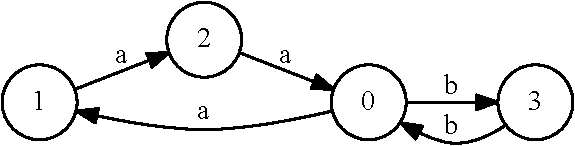
\includegraphics[width=0.45\textwidth]{pictures/input.pdf}
        &
    $

    \begin{array}{rl}
       0:& S \rightarrow a \ S \ b \\
       1:& S \rightarrow Middle \\
       2:& Middle \rightarrow a \ b
    \end{array}

    $
    \\
    Input graph
    &
    Grammar

    \end{tabular}
  \end{center}

\begin{tabular}{  c  c  c  }
      \onslide<2-4>{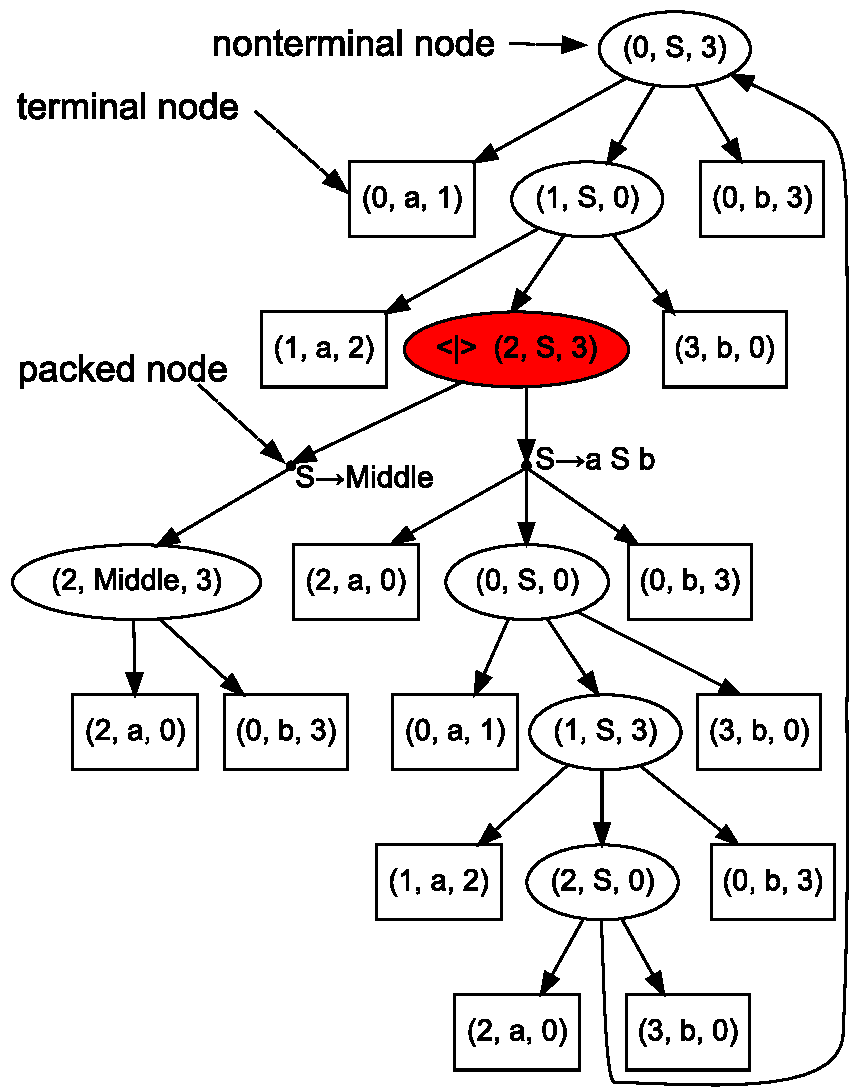
\includegraphics[height=4.5cm]{pictures/AnBn.pdf}}
    &
      \onslide<3-4>{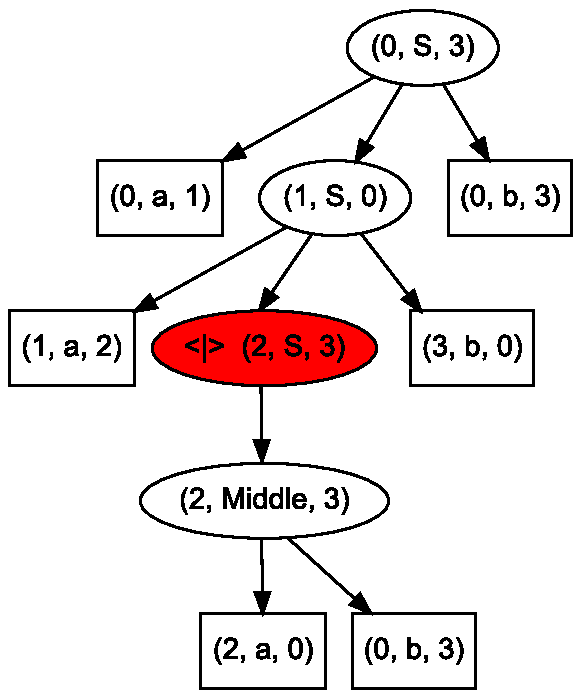
\includegraphics[height=4.5cm]{pictures/AnBn_2.pdf}}
    &
      \onslide<4>{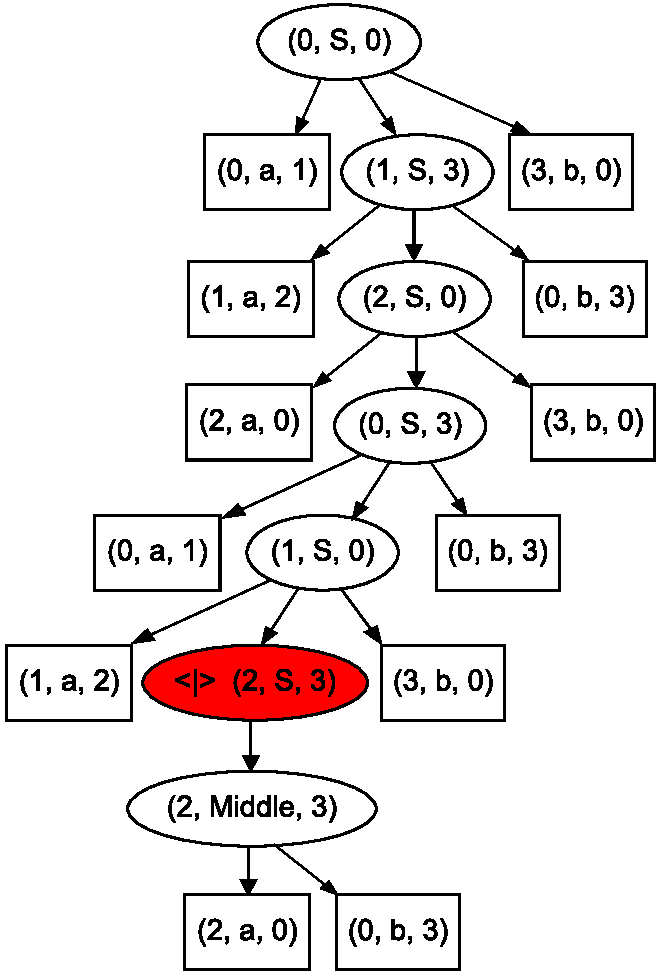
\includegraphics[height=4.5cm]{pictures/AnBn_1.pdf}}

\\
\onslide<2-4>{\small{Query result (SPPF)}}
& \onslide<3-4>{\small{Tree for $p_1$}}
& \onslide<4>{\small{Tree for $p_2$}}

\end{tabular}
%\end{center}
\end{frame}

\begin{frame}[fragile] \frametitle{Paths extraction}
\begin{center}
\begin{tabular}{  c  c  }
    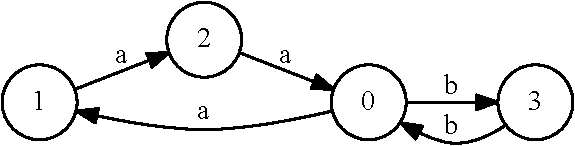
\includegraphics[width=0.45\textwidth]{pictures/input.pdf}
    &
$

\begin{array}{rl}
   0:& S \rightarrow a \ S \ b \\
   1:& S \rightarrow Middle \\
   2:& Middle \rightarrow a \ b
\end{array}

$
\end{tabular}

\begin{figure}[ht]
    \centering
        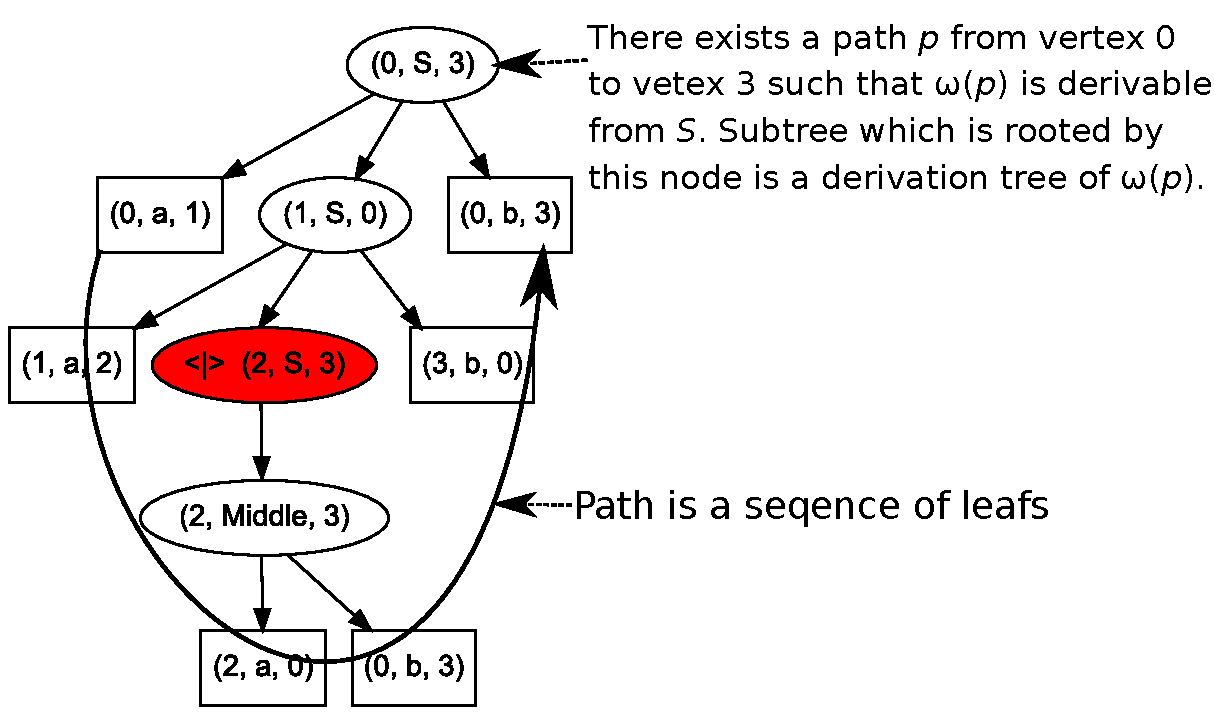
\includegraphics[width=0.68\textwidth]{pictures/AnBn_2_m.pdf}
\end{figure}
Path: $0\xrightarrow{a}1\xrightarrow{a}2\xrightarrow{a}0\xrightarrow{b}3\xrightarrow{b}0\xrightarrow{b}3$
\end{center}
\end{frame}


\begin{frame}[fragile]
  %\transwipe[direction=90]
  \frametitle{Bar-Hillel theorem}
Context-free languages are closed under intersection with regular languages
\begin{center}
\begin{tabular}{  c  c  }
    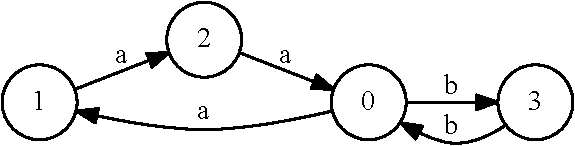
\includegraphics[width=0.35\textwidth]{pictures/input.pdf}
    &
$

\begin{array}{rl}
   0:& S \rightarrow a \ S \ b \\
   1:& S \rightarrow Middle \\
   2:& Middle \rightarrow a \ b
\end{array}

$
\\
Regular language
&
Context-free language

\end{tabular}

\vspace{0.8em}
\pause

\begin{tabular}{  c  c  }
    \raisebox{-0.5\totalheight}{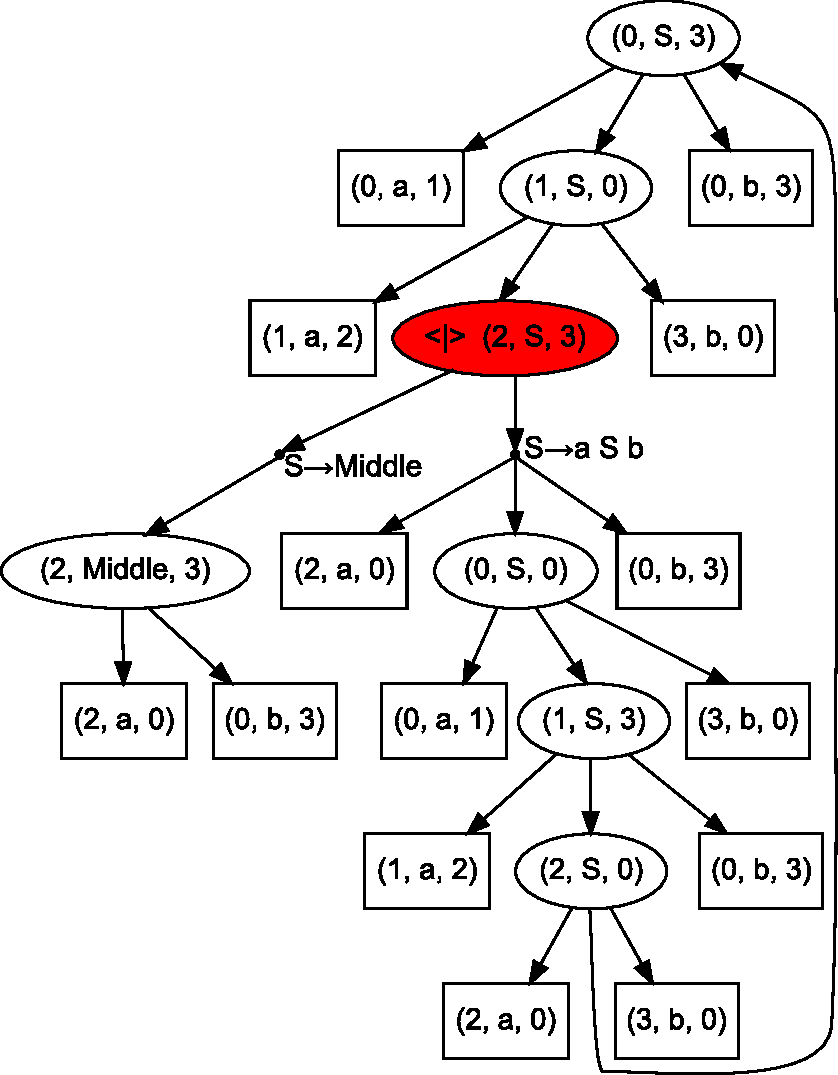
\includegraphics[width=0.32\textwidth]{pictures/AnBn_m.pdf}}
    &
\pause
$
\begin{array}{rl}
   (0,S,3) & \rightarrow (0,a,1) \ (1,S,0) \ (0,b,3) \\
   (1,S,0) & \rightarrow (1,a,2) \ (2,S,3) \ (3,b,0) \\
   (2,S,3) & \rightarrow (2,a,0) \ (0,S,0) \ (0,b,3) \\
   (2,S,3) & \rightarrow (2,Middle,3)                \\
   (0,S,0) & \rightarrow (0,a,1) \ (1,S,3) \ (3,b,0) \\
   (1,S,3) & \rightarrow (1,a,2) \ (2,S,0) \ (0,b,3) \\
   (2,S,0) & \rightarrow (2,a,0) \ (0,S,3) \ (3,b,0) \\
   (0,Middle,3) & \rightarrow (2,a,0) \ (0,b,3)  \\
\end{array}
$

\end{tabular}
\end{center}
\end{frame}

\begin{frame}[fragile] \frametitle{Our experiments}

\begin{itemize}
\item Generalized LR for CFPQ
\begin{itemize}
  \item Based on Right Nulled Generalized LR: \emph{Scott E., Johnstone A.} ``Right Nulled GLR Parsers''
  \item \emph{Ekaterina Verbitskaia, Semyon Grigorev, and Dmitry Avdyukhin.} ``Relaxed Parsing of Regular Approximations of String-Embedded Languages'' 2015
\end{itemize}

\pause

\item Generalized LL for CFPQ (\textbf{GLL})
\begin{itemize}
  \item Based on Generalized LL: \emph{Scott E., Johnstone A.} ``GLL parsing''
  \item \emph{Semyon Grigorev and Anastasiya Ragozina.} ``Context-free path querying with structural
  representation of result.'' 2017
\end{itemize}

\end{itemize}
\end{frame}

\begin{frame}[fragile] \frametitle{Query language integration}
How to integrate query language into general-purpose programming language?
\begin{itemize}
\item Transparency
\item Compositionality
\item Static error checking
\end{itemize}
\pause
\begin{itemize}
  \item String-embedded languages
  \item ORMs
  \item Combinators
\end{itemize}
\end{frame}

\begin{frame}[fragile] \frametitle{Combinators for CFPQ}
  \begin{itemize}
    \item Implemented in Scala
    \item Based on Meerkat parser combinator library: \emph{Anastasia Izmaylova, Ali Afroozeh, and Tijs van der Storm.} ``Practical, general parser combinators'' 2016
    \item \emph{Ekaterina Verbitskaia, Ilya Kirillov, Ilya Nozkin, Semyon Grigorev.} ``Parser Combinators for Context-Free Path Querying'' 2019
  \end{itemize}
\end{frame}


\begin{frame}[fragile] \frametitle{Supported combinators}
  \begin{table}[h]
  \small
  \centering
  \begin{tabular}{l@{}|l}
  \multicolumn{1}{c|}{Combinator} & \multicolumn{1}{|c}{Description} \\ \hline
  {\lstinline!a ~ b!} & sequential parsing: {\lstinline!a!} then {\lstinline!b!}   \\
  {\lstinline!a | b!} & choice: {\lstinline!a!} or {\lstinline!b!}         \\ \pause
  {\lstinline!a ?!}   & optional parsing: {\lstinline!a!} or nothing   \\
  {\lstinline!a *!}   & repetition of zero or more {\lstinline!a!} \\
  {\lstinline!a +!}   & repetition of at least one {\lstinline!a!} \\ \hline \pause
  {\lstinline!a ^ f!} & apply {\lstinline!f!} function to {\lstinline!a!} if  {\lstinline!a!} is a token \\
  {\lstinline!a ^^!}  & capture output of {\lstinline!a!} if {\lstinline!a!} is a token    \\
  {\lstinline!a & f!} & apply {\lstinline!f!} function to {\lstinline!a!} if  {\lstinline!a!} is a parser \\
  {\lstinline!a &&!}  & capture output of {\lstinline!a!} if {\lstinline!a!} is a parser    \\
  \hline
  \end{tabular}
  \end{table}

A set of functions for edges and vertices values handling.
\begin{lstlisting}
def LV(labels: String*) =
  V(e => labels.forall(e.hasLabel))
def outLE(label:String) = outE(_.label() == label)
def inLE (label:String) = inE (_.label() == label)
\end{lstlisting}
\end{frame}



\begin{frame}[fragile] \frametitle{Basic example}
  \lstset{language=scala}
  Is there a path from vertex 0 to vertex 3 which has form $a^nb^n$?
\begin{lstlisting}
val Query : Nonterminal
    = syn (LV("0") ~ S ~ LV("3"))

val S: Nonterminal
    = syn ( "a" ~ S ~ "b"
          | "a" ~ "b"
          )
\end{lstlisting}
\end{frame}

\begin{frame}[fragile] \frametitle{Example of generalization}
  \lstset{language=scala}
\begin{lstlisting}
def sameGen(brs) =
  reduceChoice(
    brs.map {case (lbr, rbr) =>
      lbr ~ syn(sameGen(brs).?) ~ rbr})
\end{lstlisting}
\pause
\begin{lstlisting}
val query1 = syn(sameGen(List(("a", "b"))))

val query2 = syn(
  sameGen(List((p1, p2),("(",")"))) ~ p3)
\end{lstlisting}

\end{frame}

\begin{frame}[fragile] \frametitle{Example of values handling}
  \lstset{language=scala}
  Actors who played in some film
  \\ In Cypher
  \begin{lstlisting}
  MATCH (m:Movie {title: 'Forrest Gump'})
        <-[:ACTS_IN]-(a:Actor)
  RETURN a.name, a.birthplace;
  \end{lstlisting}
  \vspace{0.5cm}
  In Meerkat
  \\
  \begin{lstlisting}
  val query =
    syn((
      (LV("Movie")::V(_.title == "Forrest Gump")) ~
      inLE("ACTS_IN") ~
      syn(LV("Actor") ^
            (e => (e.name, e.birthplace)))) &&)
  executeQuery(query, input)
  \end{lstlisting}

\end{frame}

\begin{frame} \frametitle{Limitations}
\begin{itemize}
  \item Overhead for the regular constraints
  \item Not exactly clear how to compute arbitrary semantics for the paths
  \begin{itemize}
    \item Paths can be lazily extracted, but in what order?
    \item Is it possible to compute some semantics in case of cycles?
  \end{itemize}
\end{itemize}
\end{frame}

\begin{frame} \frametitle{Boolean Matrix Multiplication for CFPQ}
\end{frame}


\begin{frame}
  \frametitle{Transitive Closure}
  \begin{itemize}
    \item Subset multiplication, $N_1, N_2 \subseteq N$
    \begin{itemize}
      \item $N_1 \cdot N_2 = \{A~|~\exists B \in N_1, \exists C \in N_2 \text{ such that }(A \rightarrow B C) \in P\}$
    \end{itemize}
    \item Subset addition: set-theoretic union.
  \end{itemize}

  \begin{itemize}
    \item Matrix multiplication
    \begin{itemize}
      \item Matrix of size $|V| \times |V|$
      \item Subsets of $N$ are elements
      \item $c_{i,j} = \bigcup^{n}_{k=1}{a_{i,k} \cdot b_{k,j}}$
    \end{itemize}
  \end{itemize}
  \begin{itemize}
    \item Transitive closure
  \begin{itemize}
    \item $a^{cf} = a^{(1)} \cup a^{(2)} \cup \cdots$
    \item $a^{(1)} = a$
    \item $a^{(i)} = a^{(i-1)} \cup (a^{(i-1)} \times a^{(i-1)}), ~i \ge 2$
  \end{itemize}
\end{itemize}

\end{frame}

\begin{frame} \frametitle{The algorithm}

\begin{algorithm}[H]
\begin{algorithmic}[1]
\caption{Context-free recognizer for graphs}
\label{alg:graphParse}
\Function{contextFreePathQuerying}{D, G}

    \State{$n \gets$ the number of nodes in $D$}
    \State{$E \gets$ the directed edge-relation from $D$}
    \State{$P \gets$ the set of production rules in $G$}
    \State{$T \gets$ the matrix $n \times n$ in which each element is $\varnothing$}
    \ForAll{$(i,x,j) \in E$}
    \Comment{Matrix initialization}
        \State{$T_{i,j} \gets T_{i,j} \cup \{A~|~(A \rightarrow x) \in P \}$}
    \EndFor
    \While{matrix $T$ is changing}

        \State{$T \gets T \cup (T \times T)$}
        \Comment{Transitive closure $T^{cf}$ calculation}
    \EndWhile
\State \Return $T$
\EndFunction
\end{algorithmic}
\end{algorithm}

\end{frame}

\begin{frame} \frametitle{Boolean Matrix Multiplication for CFPQ}
  \begin{itemize}
    \item The matrix for nonterminal is a set of boolean matrices
    \item Matrices multiplication can be implemented efficiently by using modern harware and high-performance libraries
  \end{itemize}
\end{frame}


\begin{frame}[fragile] \frametitle{Performance comparison setup}
We use graphs from the classical set of ontologies: \textit{skos, foaf, univ-bench, wine, pizza, etc.}
\\
\vspace{2cm}

Queries are classical variants of the same-generation query

\begin{minipage}{0.47\textwidth}
\begin{center}
   \[
\begin{array}{rl}
  &\textbf{S} \rightarrow \text{\textit{subClassOf}}^{-1} \ \textbf{S} \ \text{\textit{subClassOf}} \\
  &\textbf{S} \rightarrow \text{\textit{type}}^{-1} \ \textbf{S} \ \text{\textit{type}} \\
  &\textbf{S} \rightarrow \text{\textit{subClassOf}}^{-1} \ \text{\textit{subClassOf}} \\
  &\textbf{S} \rightarrow \text{\textit{type}}^{-1} \ \text{\textit{type}} \\
\end{array}
\]
\\
   Query 1
   \end{center}
\end{minipage}
\vspace{2cm}
\begin{minipage} {0.47\textwidth}
   \begin{center}
   \[
\begin{array}{rl}
   &\textbf{S} \rightarrow \textbf{B} \ \text{\textit{subClassOf}} \\
   &\textbf{S} \rightarrow \text{\textit{subClassOf}} \\
   &\textbf{B} \rightarrow \text{\textit{subClassOf}}^{-1} \ \textbf{B} \ \text{\textit{subClassOf}} \\
   &\textbf{B} \rightarrow \text{\textit{subClassOf}}^{-1} \ \text{\textit{subClassOf}} \\
\end{array}
\]
\\
   Query 2
\end{center}
\end{minipage}


\end{frame}


\begin{frame}[fragile]
\frametitle{Performance comparison results}
\centering
\rowcolors{1}{}{lightgray}
\begin{tabular}{  c | c | c | c | c | c | c | c }
%\hline
\textnumero & \#V & \#E & \multicolumn{3}{c|}{Query 1 (ms)} & \multicolumn{2}{c}{Query 2 (ms)} \\
\cline{4-8}
& & & CYK\footnote{Zhang, et al. ``Context-free path queries on RDF graphs.''} & GLL & GPGPU & GLL & GPGPU \\
\hline
\hline
1  & 144  & 323   & 1044    & 10   & 12  & 1   & 1 \\
2  & 129  & 351   & 6091    & 19   & 13  & 1   & 0 \\
3  & 131  & 397   & 13971   & 24   & 30  & 1   & 10 \\
4  & 179  & 413   & 20981   & 25   & 15  & 11  & 9 \\
5  & 337  & 834   & 82081   & 89   & 32  & 3   & 6 \\
6  & 291  & 685   & 515285  & 255  & 22  & 66  & 2 \\
7  & 341  & 711   & 420604  & 261  & 20  & 45  & 24 \\
8  & 671  & 2604  & 3233587 & 697  & 24  & 29  & 23 \\
9  & 733  & 2450  & 4075319 & 819  & 54  & 8   & 6 \\
10 & 6224 & 11840 & --      & 1926 & 82  & 167 & 38\\
11 & 5864 & 19600 & --      & 6246 & 185 & 46  & 21\\
12 & 5368 & 20832 & --      & 7014 & 127 & 393 & 40\\

%\hline
\end{tabular}

\end{frame}


\begin{frame}[fragile]
\frametitle{Performance comparison results}
\centering


{\setlength{\tabcolsep}{0.25em}
\rowcolors{1}{}{lightgray}
\begin{tabular}{| l | c | c | c | c | c | c | }
    \hline
    Graph              & Scipy   & M4RI     & GPU4R  & GPU\_N & GPU\_Py & CuSprs  \\
    \hline
    \hline
    \small{G5k-0.001}  & 10.352  & 0.647    & 0.113  & 0.041  & 0.216   & 5.729   \\
    \small{G10k-0.001} & 37.286  & 2.395    & 0.435  & 0.215  & 1.331   & 35.937  \\
    \small{G10k-0.01}  & 97.607  & 1.455    & 0.273  & 0.138  & 0.763   & 47.525  \\
    \small{G10k-0.1}   & 601.182 & 1.050    & 0.223  & 0.114  & 0.859   & 395.393 \\
    \small{G20k-0.001} & 150.774 & 11.025   & 1.842  & 1.274  & 6.180   & -       \\
    \small{G40k-0.001} & -       & 97.841   & 11.663 & 8.393  & 37.821  & -       \\
    \small{G80k-0.001} & -       & 1142.959 & 88.366 & 65.886 & -       & -       \\
    \hline
  \end{tabular}

}

\end{frame}


\begin{frame} \frametitle{Directions for research}
\begin{itemize}
\item Develop parallel and distributed algorithms
\item Adopt other parsing algortihms
\item Utilize other classes of languages for constraints specification
\item Investigate incremental queryes evaluation
\end{itemize}
\end{frame}

\end{document}
